\documentclass[10pt]{article}

\usepackage{amsfonts}
\usepackage{amsmath}
\usepackage{geometry}
\usepackage{xcolor,graphicx}
%\usepackage{wrapfig}
\usepackage{subcaption}
\usepackage{hyperref}
\usepackage{mathtools}


\providecommand{\e}[1]{\ensuremath{\times 10^{#1}}}

\title{Simulating the Universe}
\author{Najla Alhamadi, Michael Cock, Rebecca Halloran, Brady Metherall, Hector Robinson}

\newgeometry{margin=1in}
\setlength\parindent{0pt}

\begin{document}
\maketitle
\section{Introduction}
	In this project, our goal was to create our own realistic simulation of the universe on a cosmological scale. Our simulation starts from a redshift of 50 (start of the universe), until a redshift of 0 (current time). In addition, our simulation only considers matter and the cosmological constant as the two components of the universe. We do this by using a particle mesh technique to simulate the universe, and solve Poisson's equation to find the accelerations of particles. We step the universe forward by using a leapfrog integrator.
\section{A Very Big Box}
	Our first step was to find the parameters of our current universe, as follows: the current Hubble constant value is 73.8 km/s/Mpc; the density parameter of the cosmological constant is 0.73; the density parameter for matter is 0.27; the total density parameter is 1.02. The critical density of the universe was found to be 9.277\e{-25} kg/m$^3$ and the value of the matter density of the universe is 2.505\e{-25} kg/m$^3$. The current age of the universe was found to be 13923.769 million years. Finally, the age of the universe at z = 50 was found to be 45.813 million years. We took a cubic section of the universe with dimensions of 50x50x50 and calculated the mass of matter inside that cube to be 1.0146\e{46} kg.  
\section{Particle-Mesh Code}
 (write about the writing of the code. Reference figure \ref{fig:accel}) \\
	In this step, we built our own Particle-Mesh Code, the input is an initial conditions N-body file and the outputs are snapshots of the system at regular "timestep" intervals. The only parameter that we could manipulate is the time step. After some testing, the value of the time step was chosen to be 0.0025. The code was tested by creating two systems; the first one was to create a perfect grid of particles, evenly spaced. Since there’s no difference in density from the average value, the grid should persist throughout the simulations and that is what is observed in our results in Figure \ref{fig:order}{}. The second system was one with random initial conditions. This should result in the formations of structures in regions with higher initial density and empty space in those with lower initial density. Figure \ref{fig:randomic}{} shows the results of the second system which agrees with the expected results.       
\section{A (somewhat) Realistic Simulation}
(add how the scaling was done????????)\\ 
	In this step, we were given a set of initial conditions. The positions in this set of conditions did not match our universe size, so we had to scale them up to match our universe size. After doing this, we ran our code based off of the altered initial conditions; the results can be seen in Figure \ref{fig:control}{}. It can clearly be seen that there are regions were large structures have been formed, and that there are vast regions where there are very few particles remaining.
	
	
\section{FoF}
	One of the question we should ask about our simulation is about the structures formed; how much mass do they contain? It is difficult to define exactly where a structure ends, so to do this we implemented the ``friend-of-a-friend" method (FoF). The idea with this method, is that groups are made up of particles within a``linking length" of each other. If two particles have one or more common neighboring particles within the linking length, they are merged into a group. It checks every particle in the system and links them together into large groups. If the linking length is chosen properly, these groups will correspond to the structures seen in the simulations.\\
	To implement this, we used a software package called FoF, created by Volker Springel. We used instructions on how to implement the code from LASTRO (University of Geneva), which can be found \href{http://obswww.unige.ch/lastro/misc/TP4/doc/rst/Exercices/Ex05.html#extracting-haloes}{here}. This software provided us with infromation the groups' mass, center of mass, and size. We plotted the groups as seen in Figure \ref{fig:groups}{} to make sure they matched up with those in our control simulation. It is seen quite obviously that the groups match up with those in Figure \ref{fig:control}. The largest two groups had masses of 29\% and 22\% of the total mass.


\section{Other Questions}
	Another question we should ask is how the size of the universe affects our simulation. As can be seen in Figure \ref{fig:1boxsize}{}, the size of the universe has been shrunk to 1Mpc$^3$. We had to rescale our initial conditions to fit into this size universe, but all other conditions remained the same. The effect of this, was that all the particles collapsed into one super massive structure. The reason for this, is that there is not enough space in between particles initially for any empty regions to form. All of the separate structure formation seen in the previous simulation can not seen here.

	A further question we can ask is \ref{fig:3mass} ******INSERT QUESTION HERE******

	Another question we need to ask is what would occur if we varied the size of our grid. Varying the number of cells in our box will affect the distribution of particles in our system and therefore will affect the long-term structure of our system. In Figure \ref{fig:1ncells}, we can observe that the particles are more spread out since there are more cells to fill. In addition, when we compare the plots we can see that in our initial condition plot we have some large structure which can corresponds to galaxies and galaxies clusters whereas this is not observed in the plot with the larger number of cells. 
	
	A final alteration we can make is to increase the number of particles in our simulations. Doing this will increase the probability of interactions between the particles, since the box is still the same size. Figure \ref{fig:n64} shows our system with the increased number of particles. As we can observe the particles almost formed a one large structure, which can be explained by the fact that the average distance between the particles have decreased by the increase in the number of particles. The decrease in distance have caused the particles to form one large structure instead of forming multiple smaller structures.   



\section{Gadget}
	One further item we decided to look at was to see how our model compared to an industry used system. To do so, we looked into using the GADGET (GAlaxies with Dark matter and Gas intEracT) system.
	GADGET is a very complex system to use. It needs a lot more time to analyze the user guide and the code to really understand what is happening. We were able to download the program and run it with sample parameters that were included in the download. Instead of trying to change our plotting code to take the snapshot files or changing the snapshot files that can be read by our program, we were able to find a program that will view the snapshot files. This program ``GADGET filer viewer" is very simple to use. It opens the file to view them and you can change the colour scheme depending on the particle type. Unfortunately we were unable to play with it long enough to determine how to get a video from it. The following image is form Gadget File Viewer of two galaxies colliding.

\begin{figure*}[h]
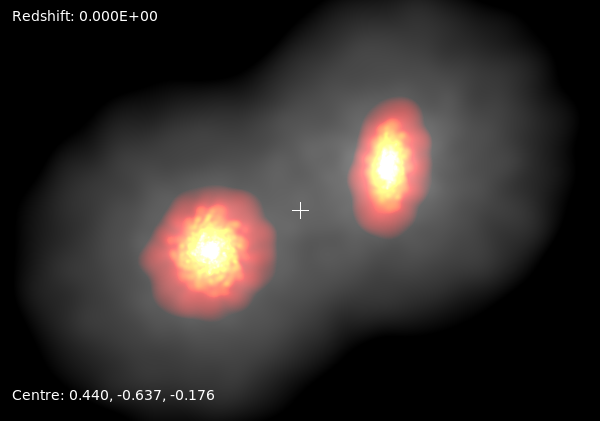
\includegraphics[width=4.5in]{gadget.png}
\centering
\end{figure*}


	After having the ability to view the snapshots we now want to run the it with our initial conditions that we had using the particle mesh so we can compare our results. We were given initial conditions to use with a parameter file that was changed to be the same as our system. Unfortunately, after many attempts the program was still giving errors about the unit mass in grams that were giving it. We had to abandon hope and attempt to try a different approach that might work better. With the unsuccessful attempt at working with Gadget we attempt to use a program we have used before, dnc. 
	To get dnc to be able to run a collapse of the universe there needs to be some changes. We need to centre a box at (0,0,0) and cut out a sphere with radius 25.  The positions will need to be scaled by the scale factor of the universe, a. This will make up for us not being able to use co-moving coordinates. Initially our system will be smaller than it is today, then it will increase to the size it is today. The initial velocity needs to be different for the initially. Normally we have it set to 0 but it needs to be in a Hubble flow which is the Hubble constant at z=50 times the position. 



\begin{figure}[htbp]
\centering
% GNUPLOT: LaTeX picture with Postscript
\begingroup
  \makeatletter
  \providecommand\color[2][]{%
    \GenericError{(gnuplot) \space\space\space\@spaces}{%
      Package color not loaded in conjunction with
      terminal option `colourtext'%
    }{See the gnuplot documentation for explanation.%
    }{Either use 'blacktext' in gnuplot or load the package
      color.sty in LaTeX.}%
    \renewcommand\color[2][]{}%
  }%
  \providecommand\includegraphics[2][]{%
    \GenericError{(gnuplot) \space\space\space\@spaces}{%
      Package graphicx or graphics not loaded%
    }{See the gnuplot documentation for explanation.%
    }{The gnuplot epslatex terminal needs graphicx.sty or graphics.sty.}%
    \renewcommand\includegraphics[2][]{}%
  }%
  \providecommand\rotatebox[2]{#2}%
  \@ifundefined{ifGPcolor}{%
    \newif\ifGPcolor
    \GPcolorfalse
  }{}%
  \@ifundefined{ifGPblacktext}{%
    \newif\ifGPblacktext
    \GPblacktexttrue
  }{}%
  % define a \g@addto@macro without @ in the name:
  \let\gplgaddtomacro\g@addto@macro
  % define empty templates for all commands taking text:
  \gdef\gplbacktext{}%
  \gdef\gplfronttext{}%
  \makeatother
  \ifGPblacktext
    % no textcolor at all
    \def\colorrgb#1{}%
    \def\colorgray#1{}%
  \else
    % gray or color?
    \ifGPcolor
      \def\colorrgb#1{\color[rgb]{#1}}%
      \def\colorgray#1{\color[gray]{#1}}%
      \expandafter\def\csname LTw\endcsname{\color{white}}%
      \expandafter\def\csname LTb\endcsname{\color{black}}%
      \expandafter\def\csname LTa\endcsname{\color{black}}%
      \expandafter\def\csname LT0\endcsname{\color[rgb]{1,0,0}}%
      \expandafter\def\csname LT1\endcsname{\color[rgb]{0,1,0}}%
      \expandafter\def\csname LT2\endcsname{\color[rgb]{0,0,1}}%
      \expandafter\def\csname LT3\endcsname{\color[rgb]{1,0,1}}%
      \expandafter\def\csname LT4\endcsname{\color[rgb]{0,1,1}}%
      \expandafter\def\csname LT5\endcsname{\color[rgb]{1,1,0}}%
      \expandafter\def\csname LT6\endcsname{\color[rgb]{0,0,0}}%
      \expandafter\def\csname LT7\endcsname{\color[rgb]{1,0.3,0}}%
      \expandafter\def\csname LT8\endcsname{\color[rgb]{0.5,0.5,0.5}}%
    \else
      % gray
      \def\colorrgb#1{\color{black}}%
      \def\colorgray#1{\color[gray]{#1}}%
      \expandafter\def\csname LTw\endcsname{\color{white}}%
      \expandafter\def\csname LTb\endcsname{\color{black}}%
      \expandafter\def\csname LTa\endcsname{\color{black}}%
      \expandafter\def\csname LT0\endcsname{\color{black}}%
      \expandafter\def\csname LT1\endcsname{\color{black}}%
      \expandafter\def\csname LT2\endcsname{\color{black}}%
      \expandafter\def\csname LT3\endcsname{\color{black}}%
      \expandafter\def\csname LT4\endcsname{\color{black}}%
      \expandafter\def\csname LT5\endcsname{\color{black}}%
      \expandafter\def\csname LT6\endcsname{\color{black}}%
      \expandafter\def\csname LT7\endcsname{\color{black}}%
      \expandafter\def\csname LT8\endcsname{\color{black}}%
    \fi
  \fi
    \setlength{\unitlength}{0.0500bp}%
    \ifx\gptboxheight\undefined%
      \newlength{\gptboxheight}%
      \newlength{\gptboxwidth}%
      \newsavebox{\gptboxtext}%
    \fi%
    \setlength{\fboxrule}{0.5pt}%
    \setlength{\fboxsep}{1pt}%
\begin{picture}(7674.00,5760.00)%
    \gplgaddtomacro\gplbacktext{%
      \csname LTb\endcsname%
      \put(1003,1433){\makebox(0,0){\strut{}$0$}}%
      \put(1698,1294){\makebox(0,0){\strut{}$10$}}%
      \put(2392,1155){\makebox(0,0){\strut{}$20$}}%
      \put(3087,1015){\makebox(0,0){\strut{}$30$}}%
      \put(3782,876){\makebox(0,0){\strut{}$40$}}%
      \put(4476,737){\makebox(0,0){\strut{}$50$}}%
      \put(4685,794){\makebox(0,0){\strut{}$0$}}%
      \put(5086,1035){\makebox(0,0){\strut{}$10$}}%
      \put(5487,1276){\makebox(0,0){\strut{}$20$}}%
      \put(5888,1518){\makebox(0,0){\strut{}$30$}}%
      \put(6289,1759){\makebox(0,0){\strut{}$40$}}%
      \put(6690,2001){\makebox(0,0){\strut{}$50$}}%
      \put(972,1529){\makebox(0,0)[r]{\strut{}$0$}}%
      \put(972,2011){\makebox(0,0)[r]{\strut{}$10$}}%
      \put(972,2494){\makebox(0,0)[r]{\strut{}$20$}}%
      \put(972,2977){\makebox(0,0)[r]{\strut{}$30$}}%
      \put(972,3459){\makebox(0,0)[r]{\strut{}$40$}}%
      \put(972,3941){\makebox(0,0)[r]{\strut{}$50$}}%
      \put(174,2735){\makebox(0,0){\strut{}$z$}}%
    }%
    \gplgaddtomacro\gplfronttext{%
      \csname LTb\endcsname%
      \put(2333,879){\makebox(0,0){\strut{}$x$}}%
      \put(6442,1261){\makebox(0,0){\strut{}$y$}}%
      \put(174,2735){\makebox(0,0){\strut{}$z$}}%
      \put(7089,2580){\makebox(0,0)[l]{\strut{}$0$}}%
      \put(7089,2819){\makebox(0,0)[l]{\strut{}$1$}}%
      \put(7089,3058){\makebox(0,0)[l]{\strut{}$2$}}%
      \put(7089,3298){\makebox(0,0)[l]{\strut{}$3$}}%
      \put(7089,3537){\makebox(0,0)[l]{\strut{}$4$}}%
      \put(7089,3776){\makebox(0,0)[l]{\strut{}$5$}}%
      \put(7089,4016){\makebox(0,0)[l]{\strut{}$6$}}%
      \put(7089,4255){\makebox(0,0)[l]{\strut{}$7$}}%
      \put(7287,3477){\makebox(0,0){\strut{}$v$}}%
    }%
    \gplbacktext
    \put(0,0){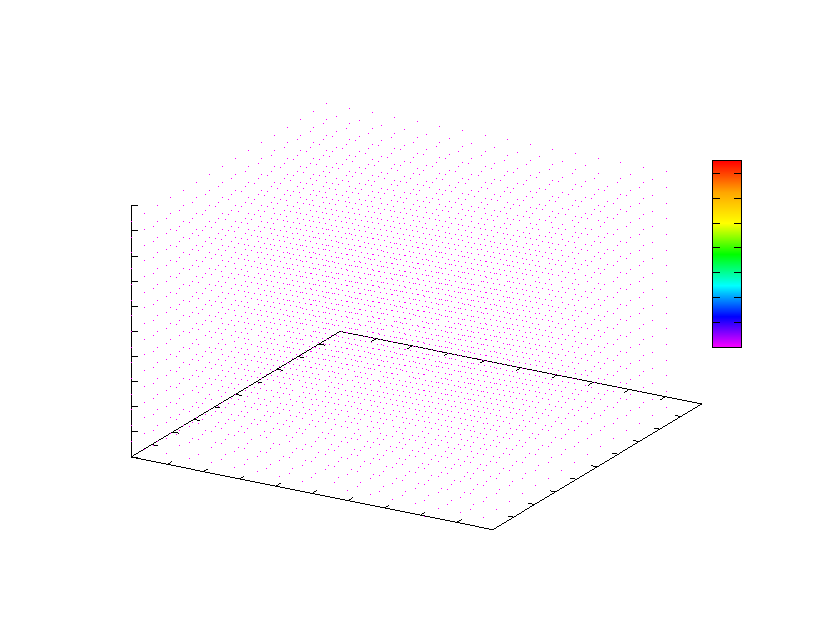
\includegraphics{Ordered}}%
    \gplfronttext
  \end{picture}%
\endgroup

\caption{Final state of system with ordered initial conditions. Nothing happened here; all particles remained motionless (Zoom in and you can see the particles!)}
\label{fig:order}
\end{figure}

\begin{figure}[htbp]
\centering
\begin{subfigure}{\textwidth}
\centering
% GNUPLOT: LaTeX picture with Postscript
\begingroup
  \makeatletter
  \providecommand\color[2][]{%
    \GenericError{(gnuplot) \space\space\space\@spaces}{%
      Package color not loaded in conjunction with
      terminal option `colourtext'%
    }{See the gnuplot documentation for explanation.%
    }{Either use 'blacktext' in gnuplot or load the package
      color.sty in LaTeX.}%
    \renewcommand\color[2][]{}%
  }%
  \providecommand\includegraphics[2][]{%
    \GenericError{(gnuplot) \space\space\space\@spaces}{%
      Package graphicx or graphics not loaded%
    }{See the gnuplot documentation for explanation.%
    }{The gnuplot epslatex terminal needs graphicx.sty or graphics.sty.}%
    \renewcommand\includegraphics[2][]{}%
  }%
  \providecommand\rotatebox[2]{#2}%
  \@ifundefined{ifGPcolor}{%
    \newif\ifGPcolor
    \GPcolorfalse
  }{}%
  \@ifundefined{ifGPblacktext}{%
    \newif\ifGPblacktext
    \GPblacktexttrue
  }{}%
  % define a \g@addto@macro without @ in the name:
  \let\gplgaddtomacro\g@addto@macro
  % define empty templates for all commands taking text:
  \gdef\gplbacktext{}%
  \gdef\gplfronttext{}%
  \makeatother
  \ifGPblacktext
    % no textcolor at all
    \def\colorrgb#1{}%
    \def\colorgray#1{}%
  \else
    % gray or color?
    \ifGPcolor
      \def\colorrgb#1{\color[rgb]{#1}}%
      \def\colorgray#1{\color[gray]{#1}}%
      \expandafter\def\csname LTw\endcsname{\color{white}}%
      \expandafter\def\csname LTb\endcsname{\color{black}}%
      \expandafter\def\csname LTa\endcsname{\color{black}}%
      \expandafter\def\csname LT0\endcsname{\color[rgb]{1,0,0}}%
      \expandafter\def\csname LT1\endcsname{\color[rgb]{0,1,0}}%
      \expandafter\def\csname LT2\endcsname{\color[rgb]{0,0,1}}%
      \expandafter\def\csname LT3\endcsname{\color[rgb]{1,0,1}}%
      \expandafter\def\csname LT4\endcsname{\color[rgb]{0,1,1}}%
      \expandafter\def\csname LT5\endcsname{\color[rgb]{1,1,0}}%
      \expandafter\def\csname LT6\endcsname{\color[rgb]{0,0,0}}%
      \expandafter\def\csname LT7\endcsname{\color[rgb]{1,0.3,0}}%
      \expandafter\def\csname LT8\endcsname{\color[rgb]{0.5,0.5,0.5}}%
    \else
      % gray
      \def\colorrgb#1{\color{black}}%
      \def\colorgray#1{\color[gray]{#1}}%
      \expandafter\def\csname LTw\endcsname{\color{white}}%
      \expandafter\def\csname LTb\endcsname{\color{black}}%
      \expandafter\def\csname LTa\endcsname{\color{black}}%
      \expandafter\def\csname LT0\endcsname{\color{black}}%
      \expandafter\def\csname LT1\endcsname{\color{black}}%
      \expandafter\def\csname LT2\endcsname{\color{black}}%
      \expandafter\def\csname LT3\endcsname{\color{black}}%
      \expandafter\def\csname LT4\endcsname{\color{black}}%
      \expandafter\def\csname LT5\endcsname{\color{black}}%
      \expandafter\def\csname LT6\endcsname{\color{black}}%
      \expandafter\def\csname LT7\endcsname{\color{black}}%
      \expandafter\def\csname LT8\endcsname{\color{black}}%
    \fi
  \fi
    \setlength{\unitlength}{0.0500bp}%
    \ifx\gptboxheight\undefined%
      \newlength{\gptboxheight}%
      \newlength{\gptboxwidth}%
      \newsavebox{\gptboxtext}%
    \fi%
    \setlength{\fboxrule}{0.5pt}%
    \setlength{\fboxsep}{1pt}%
\begin{picture}(7674.00,5760.00)%
    \gplgaddtomacro\gplbacktext{%
      \csname LTb\endcsname%
      \put(990,704){\makebox(0,0)[r]{\strut{}$0$}}%
      \put(990,1662){\makebox(0,0)[r]{\strut{}$10$}}%
      \put(990,2620){\makebox(0,0)[r]{\strut{}$20$}}%
      \put(990,3579){\makebox(0,0)[r]{\strut{}$30$}}%
      \put(990,4537){\makebox(0,0)[r]{\strut{}$40$}}%
      \put(990,5495){\makebox(0,0)[r]{\strut{}$50$}}%
      \put(1122,484){\makebox(0,0){\strut{}$0$}}%
      \put(2080,484){\makebox(0,0){\strut{}$10$}}%
      \put(3038,484){\makebox(0,0){\strut{}$20$}}%
      \put(3997,484){\makebox(0,0){\strut{}$30$}}%
      \put(4955,484){\makebox(0,0){\strut{}$40$}}%
      \put(5913,484){\makebox(0,0){\strut{}$50$}}%
    }%
    \gplgaddtomacro\gplfronttext{%
      \csname LTb\endcsname%
      \put(484,3099){\rotatebox{-270}{\makebox(0,0){\strut{}$y$}}}%
      \put(3517,154){\makebox(0,0){\strut{}$x$}}%
      \csname LTb\endcsname%
      \put(6404,704){\makebox(0,0)[l]{\strut{}$0$}}%
      \put(6404,1342){\makebox(0,0)[l]{\strut{}$2$}}%
      \put(6404,1981){\makebox(0,0)[l]{\strut{}$4$}}%
      \put(6404,2620){\makebox(0,0)[l]{\strut{}$6$}}%
      \put(6404,3259){\makebox(0,0)[l]{\strut{}$8$}}%
      \put(6404,3898){\makebox(0,0)[l]{\strut{}$10$}}%
      \put(6404,4536){\makebox(0,0)[l]{\strut{}$12$}}%
      \put(6404,5175){\makebox(0,0)[l]{\strut{}$14$}}%
      \put(6734,3099){\makebox(0,0){\strut{}$v$}}%
    }%
    \gplbacktext
    \put(0,0){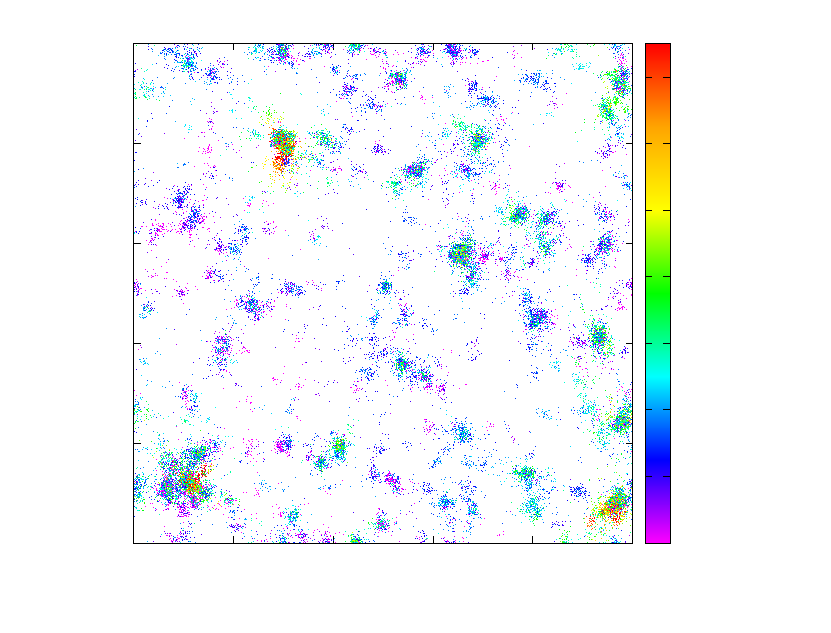
\includegraphics{Random2D}}%
    \gplfronttext
  \end{picture}%
\endgroup

\end{subfigure} \\
\begin{subfigure}{\textwidth}
\centering
% GNUPLOT: LaTeX picture with Postscript
\begingroup
  \makeatletter
  \providecommand\color[2][]{%
    \GenericError{(gnuplot) \space\space\space\@spaces}{%
      Package color not loaded in conjunction with
      terminal option `colourtext'%
    }{See the gnuplot documentation for explanation.%
    }{Either use 'blacktext' in gnuplot or load the package
      color.sty in LaTeX.}%
    \renewcommand\color[2][]{}%
  }%
  \providecommand\includegraphics[2][]{%
    \GenericError{(gnuplot) \space\space\space\@spaces}{%
      Package graphicx or graphics not loaded%
    }{See the gnuplot documentation for explanation.%
    }{The gnuplot epslatex terminal needs graphicx.sty or graphics.sty.}%
    \renewcommand\includegraphics[2][]{}%
  }%
  \providecommand\rotatebox[2]{#2}%
  \@ifundefined{ifGPcolor}{%
    \newif\ifGPcolor
    \GPcolorfalse
  }{}%
  \@ifundefined{ifGPblacktext}{%
    \newif\ifGPblacktext
    \GPblacktexttrue
  }{}%
  % define a \g@addto@macro without @ in the name:
  \let\gplgaddtomacro\g@addto@macro
  % define empty templates for all commands taking text:
  \gdef\gplbacktext{}%
  \gdef\gplfronttext{}%
  \makeatother
  \ifGPblacktext
    % no textcolor at all
    \def\colorrgb#1{}%
    \def\colorgray#1{}%
  \else
    % gray or color?
    \ifGPcolor
      \def\colorrgb#1{\color[rgb]{#1}}%
      \def\colorgray#1{\color[gray]{#1}}%
      \expandafter\def\csname LTw\endcsname{\color{white}}%
      \expandafter\def\csname LTb\endcsname{\color{black}}%
      \expandafter\def\csname LTa\endcsname{\color{black}}%
      \expandafter\def\csname LT0\endcsname{\color[rgb]{1,0,0}}%
      \expandafter\def\csname LT1\endcsname{\color[rgb]{0,1,0}}%
      \expandafter\def\csname LT2\endcsname{\color[rgb]{0,0,1}}%
      \expandafter\def\csname LT3\endcsname{\color[rgb]{1,0,1}}%
      \expandafter\def\csname LT4\endcsname{\color[rgb]{0,1,1}}%
      \expandafter\def\csname LT5\endcsname{\color[rgb]{1,1,0}}%
      \expandafter\def\csname LT6\endcsname{\color[rgb]{0,0,0}}%
      \expandafter\def\csname LT7\endcsname{\color[rgb]{1,0.3,0}}%
      \expandafter\def\csname LT8\endcsname{\color[rgb]{0.5,0.5,0.5}}%
    \else
      % gray
      \def\colorrgb#1{\color{black}}%
      \def\colorgray#1{\color[gray]{#1}}%
      \expandafter\def\csname LTw\endcsname{\color{white}}%
      \expandafter\def\csname LTb\endcsname{\color{black}}%
      \expandafter\def\csname LTa\endcsname{\color{black}}%
      \expandafter\def\csname LT0\endcsname{\color{black}}%
      \expandafter\def\csname LT1\endcsname{\color{black}}%
      \expandafter\def\csname LT2\endcsname{\color{black}}%
      \expandafter\def\csname LT3\endcsname{\color{black}}%
      \expandafter\def\csname LT4\endcsname{\color{black}}%
      \expandafter\def\csname LT5\endcsname{\color{black}}%
      \expandafter\def\csname LT6\endcsname{\color{black}}%
      \expandafter\def\csname LT7\endcsname{\color{black}}%
      \expandafter\def\csname LT8\endcsname{\color{black}}%
    \fi
  \fi
    \setlength{\unitlength}{0.0500bp}%
    \ifx\gptboxheight\undefined%
      \newlength{\gptboxheight}%
      \newlength{\gptboxwidth}%
      \newsavebox{\gptboxtext}%
    \fi%
    \setlength{\fboxrule}{0.5pt}%
    \setlength{\fboxsep}{1pt}%
\begin{picture}(7674.00,5760.00)%
    \gplgaddtomacro\gplbacktext{%
      \csname LTb\endcsname%
      \put(1003,1433){\makebox(0,0){\strut{}$0$}}%
      \put(1698,1294){\makebox(0,0){\strut{}$10$}}%
      \put(2392,1155){\makebox(0,0){\strut{}$20$}}%
      \put(3087,1015){\makebox(0,0){\strut{}$30$}}%
      \put(3782,876){\makebox(0,0){\strut{}$40$}}%
      \put(4476,737){\makebox(0,0){\strut{}$50$}}%
      \put(4685,794){\makebox(0,0){\strut{}$0$}}%
      \put(5086,1035){\makebox(0,0){\strut{}$10$}}%
      \put(5487,1276){\makebox(0,0){\strut{}$20$}}%
      \put(5888,1518){\makebox(0,0){\strut{}$30$}}%
      \put(6289,1759){\makebox(0,0){\strut{}$40$}}%
      \put(6690,2001){\makebox(0,0){\strut{}$50$}}%
      \put(972,1529){\makebox(0,0)[r]{\strut{}$0$}}%
      \put(972,2011){\makebox(0,0)[r]{\strut{}$10$}}%
      \put(972,2494){\makebox(0,0)[r]{\strut{}$20$}}%
      \put(972,2977){\makebox(0,0)[r]{\strut{}$30$}}%
      \put(972,3459){\makebox(0,0)[r]{\strut{}$40$}}%
      \put(972,3941){\makebox(0,0)[r]{\strut{}$50$}}%
      \put(174,2735){\makebox(0,0){\strut{}$z$}}%
    }%
    \gplgaddtomacro\gplfronttext{%
      \csname LTb\endcsname%
      \put(2333,879){\makebox(0,0){\strut{}$x$}}%
      \put(6442,1261){\makebox(0,0){\strut{}$y$}}%
      \put(174,2735){\makebox(0,0){\strut{}$z$}}%
      \put(7089,2580){\makebox(0,0)[l]{\strut{}$0$}}%
      \put(7089,2819){\makebox(0,0)[l]{\strut{}$2$}}%
      \put(7089,3058){\makebox(0,0)[l]{\strut{}$4$}}%
      \put(7089,3298){\makebox(0,0)[l]{\strut{}$6$}}%
      \put(7089,3537){\makebox(0,0)[l]{\strut{}$8$}}%
      \put(7089,3776){\makebox(0,0)[l]{\strut{}$10$}}%
      \put(7089,4016){\makebox(0,0)[l]{\strut{}$12$}}%
      \put(7089,4255){\makebox(0,0)[l]{\strut{}$14$}}%
      \put(7419,3477){\makebox(0,0){\strut{}$v$}}%
    }%
    \gplbacktext
    \put(0,0){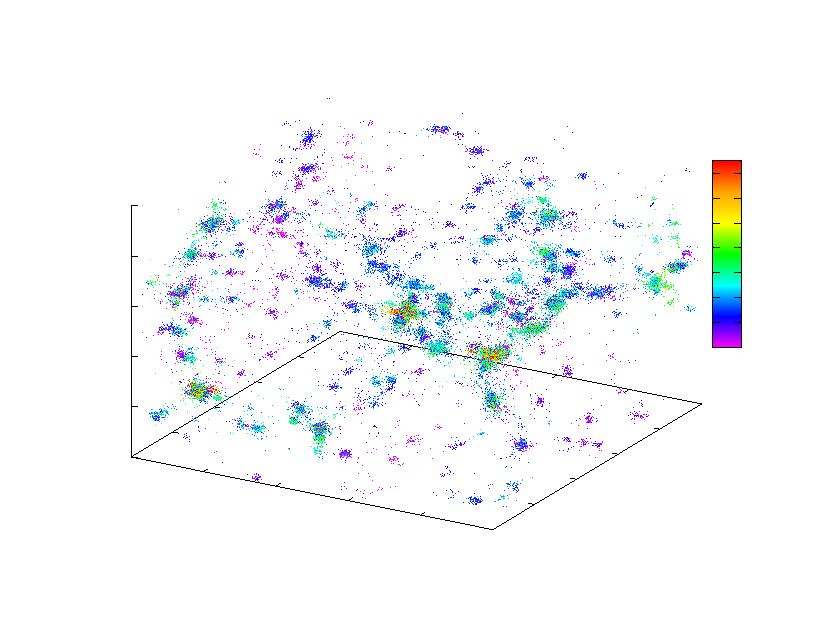
\includegraphics{Random3D}}%
    \gplfronttext
  \end{picture}%
\endgroup

\end{subfigure}
\caption{Final state of system with random initial conditions, shown in 2D and 3D. Color corresponds to particle velocity.}
\label{fig:randomic}
\end{figure}

\begin{figure}[htbp]
\centering
\begin{subfigure}{\textwidth}
\centering
% GNUPLOT: LaTeX picture with Postscript
\begingroup
  \makeatletter
  \providecommand\color[2][]{%
    \GenericError{(gnuplot) \space\space\space\@spaces}{%
      Package color not loaded in conjunction with
      terminal option `colourtext'%
    }{See the gnuplot documentation for explanation.%
    }{Either use 'blacktext' in gnuplot or load the package
      color.sty in LaTeX.}%
    \renewcommand\color[2][]{}%
  }%
  \providecommand\includegraphics[2][]{%
    \GenericError{(gnuplot) \space\space\space\@spaces}{%
      Package graphicx or graphics not loaded%
    }{See the gnuplot documentation for explanation.%
    }{The gnuplot epslatex terminal needs graphicx.sty or graphics.sty.}%
    \renewcommand\includegraphics[2][]{}%
  }%
  \providecommand\rotatebox[2]{#2}%
  \@ifundefined{ifGPcolor}{%
    \newif\ifGPcolor
    \GPcolorfalse
  }{}%
  \@ifundefined{ifGPblacktext}{%
    \newif\ifGPblacktext
    \GPblacktexttrue
  }{}%
  % define a \g@addto@macro without @ in the name:
  \let\gplgaddtomacro\g@addto@macro
  % define empty templates for all commands taking text:
  \gdef\gplbacktext{}%
  \gdef\gplfronttext{}%
  \makeatother
  \ifGPblacktext
    % no textcolor at all
    \def\colorrgb#1{}%
    \def\colorgray#1{}%
  \else
    % gray or color?
    \ifGPcolor
      \def\colorrgb#1{\color[rgb]{#1}}%
      \def\colorgray#1{\color[gray]{#1}}%
      \expandafter\def\csname LTw\endcsname{\color{white}}%
      \expandafter\def\csname LTb\endcsname{\color{black}}%
      \expandafter\def\csname LTa\endcsname{\color{black}}%
      \expandafter\def\csname LT0\endcsname{\color[rgb]{1,0,0}}%
      \expandafter\def\csname LT1\endcsname{\color[rgb]{0,1,0}}%
      \expandafter\def\csname LT2\endcsname{\color[rgb]{0,0,1}}%
      \expandafter\def\csname LT3\endcsname{\color[rgb]{1,0,1}}%
      \expandafter\def\csname LT4\endcsname{\color[rgb]{0,1,1}}%
      \expandafter\def\csname LT5\endcsname{\color[rgb]{1,1,0}}%
      \expandafter\def\csname LT6\endcsname{\color[rgb]{0,0,0}}%
      \expandafter\def\csname LT7\endcsname{\color[rgb]{1,0.3,0}}%
      \expandafter\def\csname LT8\endcsname{\color[rgb]{0.5,0.5,0.5}}%
    \else
      % gray
      \def\colorrgb#1{\color{black}}%
      \def\colorgray#1{\color[gray]{#1}}%
      \expandafter\def\csname LTw\endcsname{\color{white}}%
      \expandafter\def\csname LTb\endcsname{\color{black}}%
      \expandafter\def\csname LTa\endcsname{\color{black}}%
      \expandafter\def\csname LT0\endcsname{\color{black}}%
      \expandafter\def\csname LT1\endcsname{\color{black}}%
      \expandafter\def\csname LT2\endcsname{\color{black}}%
      \expandafter\def\csname LT3\endcsname{\color{black}}%
      \expandafter\def\csname LT4\endcsname{\color{black}}%
      \expandafter\def\csname LT5\endcsname{\color{black}}%
      \expandafter\def\csname LT6\endcsname{\color{black}}%
      \expandafter\def\csname LT7\endcsname{\color{black}}%
      \expandafter\def\csname LT8\endcsname{\color{black}}%
    \fi
  \fi
    \setlength{\unitlength}{0.0500bp}%
    \ifx\gptboxheight\undefined%
      \newlength{\gptboxheight}%
      \newlength{\gptboxwidth}%
      \newsavebox{\gptboxtext}%
    \fi%
    \setlength{\fboxrule}{0.5pt}%
    \setlength{\fboxsep}{1pt}%
\begin{picture}(7674.00,5760.00)%
    \gplgaddtomacro\gplbacktext{%
      \csname LTb\endcsname%
      \put(990,704){\makebox(0,0)[r]{\strut{}$0$}}%
      \put(990,1662){\makebox(0,0)[r]{\strut{}$10$}}%
      \put(990,2620){\makebox(0,0)[r]{\strut{}$20$}}%
      \put(990,3579){\makebox(0,0)[r]{\strut{}$30$}}%
      \put(990,4537){\makebox(0,0)[r]{\strut{}$40$}}%
      \put(990,5495){\makebox(0,0)[r]{\strut{}$50$}}%
      \put(1122,484){\makebox(0,0){\strut{}$0$}}%
      \put(2080,484){\makebox(0,0){\strut{}$10$}}%
      \put(3038,484){\makebox(0,0){\strut{}$20$}}%
      \put(3997,484){\makebox(0,0){\strut{}$30$}}%
      \put(4955,484){\makebox(0,0){\strut{}$40$}}%
      \put(5913,484){\makebox(0,0){\strut{}$50$}}%
    }%
    \gplgaddtomacro\gplfronttext{%
      \csname LTb\endcsname%
      \put(484,3099){\makebox(0,0){\strut{}$y$}}%
      \put(3517,154){\makebox(0,0){\strut{}$x$}}%
      \csname LTb\endcsname%
      \put(6404,704){\makebox(0,0)[l]{\strut{}$0$}}%
      \put(6404,1183){\makebox(0,0)[l]{\strut{}$5$}}%
      \put(6404,1662){\makebox(0,0)[l]{\strut{}$10$}}%
      \put(6404,2141){\makebox(0,0)[l]{\strut{}$15$}}%
      \put(6404,2620){\makebox(0,0)[l]{\strut{}$20$}}%
      \put(6404,3099){\makebox(0,0)[l]{\strut{}$25$}}%
      \put(6404,3578){\makebox(0,0)[l]{\strut{}$30$}}%
      \put(6404,4057){\makebox(0,0)[l]{\strut{}$35$}}%
      \put(6404,4536){\makebox(0,0)[l]{\strut{}$40$}}%
      \put(6404,5015){\makebox(0,0)[l]{\strut{}$45$}}%
      \put(6404,5495){\makebox(0,0)[l]{\strut{}$50$}}%
      \put(6734,3099){\makebox(0,0){\strut{}$z$}}%
    }%
    \gplbacktext
    \put(0,0){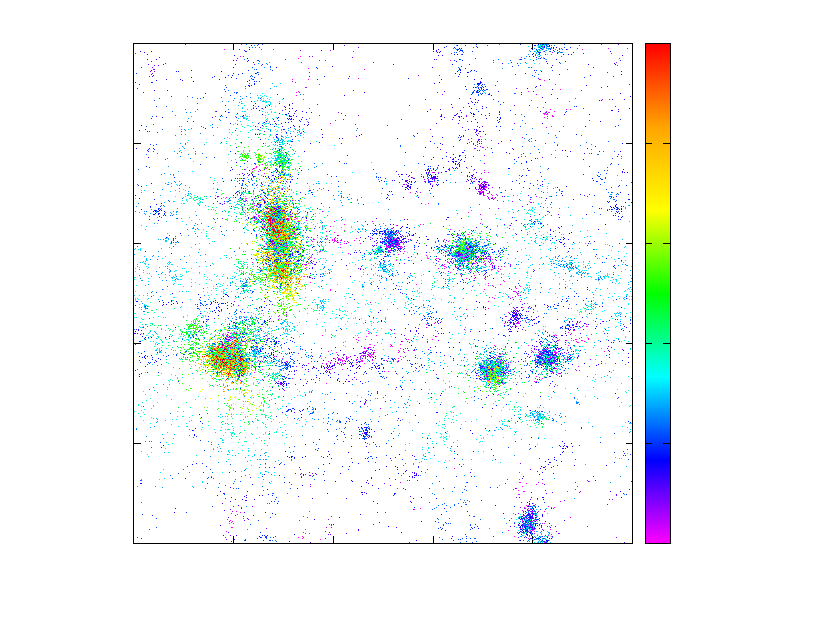
\includegraphics{Control}}%
    \gplfronttext
  \end{picture}%
\endgroup

\caption{Top-down view.}
\end{subfigure} \\
\begin{subfigure}{\textwidth}
\centering
% GNUPLOT: LaTeX picture with Postscript
\begingroup
  \makeatletter
  \providecommand\color[2][]{%
    \GenericError{(gnuplot) \space\space\space\@spaces}{%
      Package color not loaded in conjunction with
      terminal option `colourtext'%
    }{See the gnuplot documentation for explanation.%
    }{Either use 'blacktext' in gnuplot or load the package
      color.sty in LaTeX.}%
    \renewcommand\color[2][]{}%
  }%
  \providecommand\includegraphics[2][]{%
    \GenericError{(gnuplot) \space\space\space\@spaces}{%
      Package graphicx or graphics not loaded%
    }{See the gnuplot documentation for explanation.%
    }{The gnuplot epslatex terminal needs graphicx.sty or graphics.sty.}%
    \renewcommand\includegraphics[2][]{}%
  }%
  \providecommand\rotatebox[2]{#2}%
  \@ifundefined{ifGPcolor}{%
    \newif\ifGPcolor
    \GPcolorfalse
  }{}%
  \@ifundefined{ifGPblacktext}{%
    \newif\ifGPblacktext
    \GPblacktexttrue
  }{}%
  % define a \g@addto@macro without @ in the name:
  \let\gplgaddtomacro\g@addto@macro
  % define empty templates for all commands taking text:
  \gdef\gplbacktext{}%
  \gdef\gplfronttext{}%
  \makeatother
  \ifGPblacktext
    % no textcolor at all
    \def\colorrgb#1{}%
    \def\colorgray#1{}%
  \else
    % gray or color?
    \ifGPcolor
      \def\colorrgb#1{\color[rgb]{#1}}%
      \def\colorgray#1{\color[gray]{#1}}%
      \expandafter\def\csname LTw\endcsname{\color{white}}%
      \expandafter\def\csname LTb\endcsname{\color{black}}%
      \expandafter\def\csname LTa\endcsname{\color{black}}%
      \expandafter\def\csname LT0\endcsname{\color[rgb]{1,0,0}}%
      \expandafter\def\csname LT1\endcsname{\color[rgb]{0,1,0}}%
      \expandafter\def\csname LT2\endcsname{\color[rgb]{0,0,1}}%
      \expandafter\def\csname LT3\endcsname{\color[rgb]{1,0,1}}%
      \expandafter\def\csname LT4\endcsname{\color[rgb]{0,1,1}}%
      \expandafter\def\csname LT5\endcsname{\color[rgb]{1,1,0}}%
      \expandafter\def\csname LT6\endcsname{\color[rgb]{0,0,0}}%
      \expandafter\def\csname LT7\endcsname{\color[rgb]{1,0.3,0}}%
      \expandafter\def\csname LT8\endcsname{\color[rgb]{0.5,0.5,0.5}}%
    \else
      % gray
      \def\colorrgb#1{\color{black}}%
      \def\colorgray#1{\color[gray]{#1}}%
      \expandafter\def\csname LTw\endcsname{\color{white}}%
      \expandafter\def\csname LTb\endcsname{\color{black}}%
      \expandafter\def\csname LTa\endcsname{\color{black}}%
      \expandafter\def\csname LT0\endcsname{\color{black}}%
      \expandafter\def\csname LT1\endcsname{\color{black}}%
      \expandafter\def\csname LT2\endcsname{\color{black}}%
      \expandafter\def\csname LT3\endcsname{\color{black}}%
      \expandafter\def\csname LT4\endcsname{\color{black}}%
      \expandafter\def\csname LT5\endcsname{\color{black}}%
      \expandafter\def\csname LT6\endcsname{\color{black}}%
      \expandafter\def\csname LT7\endcsname{\color{black}}%
      \expandafter\def\csname LT8\endcsname{\color{black}}%
    \fi
  \fi
    \setlength{\unitlength}{0.0500bp}%
    \ifx\gptboxheight\undefined%
      \newlength{\gptboxheight}%
      \newlength{\gptboxwidth}%
      \newsavebox{\gptboxtext}%
    \fi%
    \setlength{\fboxrule}{0.5pt}%
    \setlength{\fboxsep}{1pt}%
\begin{picture}(7674.00,5760.00)%
    \gplgaddtomacro\gplbacktext{%
      \csname LTb\endcsname%
      \put(1003,1433){\makebox(0,0){\strut{}$0$}}%
      \put(1698,1294){\makebox(0,0){\strut{}$10$}}%
      \put(2392,1155){\makebox(0,0){\strut{}$20$}}%
      \put(3087,1015){\makebox(0,0){\strut{}$30$}}%
      \put(3782,876){\makebox(0,0){\strut{}$40$}}%
      \put(4476,737){\makebox(0,0){\strut{}$50$}}%
      \put(4685,794){\makebox(0,0){\strut{}$0$}}%
      \put(5086,1035){\makebox(0,0){\strut{}$10$}}%
      \put(5487,1276){\makebox(0,0){\strut{}$20$}}%
      \put(5888,1518){\makebox(0,0){\strut{}$30$}}%
      \put(6289,1759){\makebox(0,0){\strut{}$40$}}%
      \put(6690,2001){\makebox(0,0){\strut{}$50$}}%
      \put(972,1529){\makebox(0,0)[r]{\strut{}$0$}}%
      \put(972,2011){\makebox(0,0)[r]{\strut{}$10$}}%
      \put(972,2494){\makebox(0,0)[r]{\strut{}$20$}}%
      \put(972,2977){\makebox(0,0)[r]{\strut{}$30$}}%
      \put(972,3459){\makebox(0,0)[r]{\strut{}$40$}}%
      \put(972,3941){\makebox(0,0)[r]{\strut{}$50$}}%
    }%
    \gplgaddtomacro\gplfronttext{%
      \csname LTb\endcsname%
      \put(2333,879){\makebox(0,0){\strut{}$x$}}%
      \put(6442,1261){\makebox(0,0){\strut{}$y$}}%
      \put(7089,2580){\makebox(0,0)[l]{\strut{}$0$}}%
      \put(7089,2759){\makebox(0,0)[l]{\strut{}$5$}}%
      \put(7089,2939){\makebox(0,0)[l]{\strut{}$10$}}%
      \put(7089,3118){\makebox(0,0)[l]{\strut{}$15$}}%
      \put(7089,3298){\makebox(0,0)[l]{\strut{}$20$}}%
      \put(7089,3477){\makebox(0,0)[l]{\strut{}$25$}}%
      \put(7089,3657){\makebox(0,0)[l]{\strut{}$30$}}%
      \put(7089,3836){\makebox(0,0)[l]{\strut{}$35$}}%
      \put(7089,4016){\makebox(0,0)[l]{\strut{}$40$}}%
      \put(7089,4195){\makebox(0,0)[l]{\strut{}$45$}}%
      \put(7089,4375){\makebox(0,0)[l]{\strut{}$50$}}%
      \put(7419,3477){\makebox(0,0){\strut{}$z$}}%
    }%
    \gplbacktext
    \put(0,0){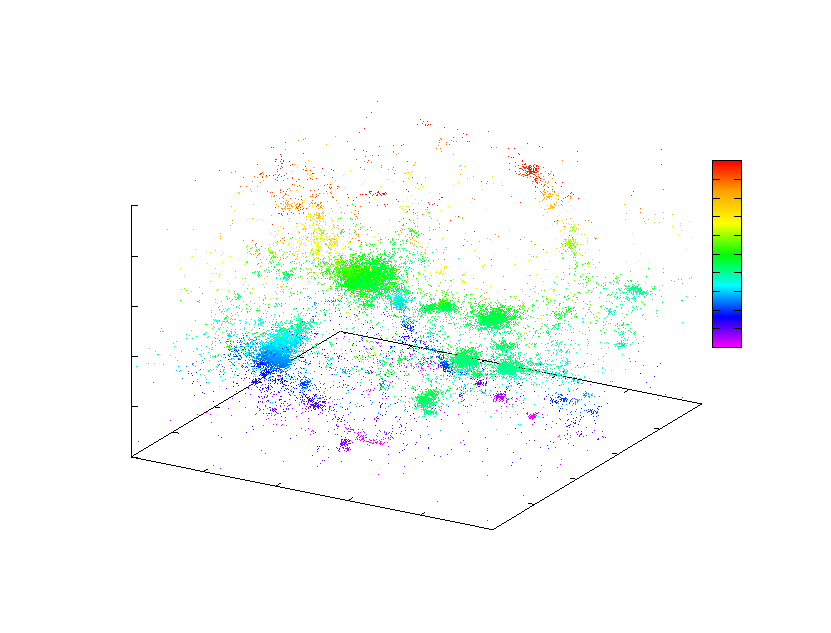
\includegraphics{Control3D}}%
    \gplfronttext
  \end{picture}%
\endgroup

\caption{3D view.}
\end{subfigure}
\caption{Control simulation.}
\label{fig:control}
\end{figure}

\begin{figure}[htbp]
\centering
% GNUPLOT: LaTeX picture with Postscript
\begingroup
  \makeatletter
  \providecommand\color[2][]{%
    \GenericError{(gnuplot) \space\space\space\@spaces}{%
      Package color not loaded in conjunction with
      terminal option `colourtext'%
    }{See the gnuplot documentation for explanation.%
    }{Either use 'blacktext' in gnuplot or load the package
      color.sty in LaTeX.}%
    \renewcommand\color[2][]{}%
  }%
  \providecommand\includegraphics[2][]{%
    \GenericError{(gnuplot) \space\space\space\@spaces}{%
      Package graphicx or graphics not loaded%
    }{See the gnuplot documentation for explanation.%
    }{The gnuplot epslatex terminal needs graphicx.sty or graphics.sty.}%
    \renewcommand\includegraphics[2][]{}%
  }%
  \providecommand\rotatebox[2]{#2}%
  \@ifundefined{ifGPcolor}{%
    \newif\ifGPcolor
    \GPcolorfalse
  }{}%
  \@ifundefined{ifGPblacktext}{%
    \newif\ifGPblacktext
    \GPblacktexttrue
  }{}%
  % define a \g@addto@macro without @ in the name:
  \let\gplgaddtomacro\g@addto@macro
  % define empty templates for all commands taking text:
  \gdef\gplbacktext{}%
  \gdef\gplfronttext{}%
  \makeatother
  \ifGPblacktext
    % no textcolor at all
    \def\colorrgb#1{}%
    \def\colorgray#1{}%
  \else
    % gray or color?
    \ifGPcolor
      \def\colorrgb#1{\color[rgb]{#1}}%
      \def\colorgray#1{\color[gray]{#1}}%
      \expandafter\def\csname LTw\endcsname{\color{white}}%
      \expandafter\def\csname LTb\endcsname{\color{black}}%
      \expandafter\def\csname LTa\endcsname{\color{black}}%
      \expandafter\def\csname LT0\endcsname{\color[rgb]{1,0,0}}%
      \expandafter\def\csname LT1\endcsname{\color[rgb]{0,1,0}}%
      \expandafter\def\csname LT2\endcsname{\color[rgb]{0,0,1}}%
      \expandafter\def\csname LT3\endcsname{\color[rgb]{1,0,1}}%
      \expandafter\def\csname LT4\endcsname{\color[rgb]{0,1,1}}%
      \expandafter\def\csname LT5\endcsname{\color[rgb]{1,1,0}}%
      \expandafter\def\csname LT6\endcsname{\color[rgb]{0,0,0}}%
      \expandafter\def\csname LT7\endcsname{\color[rgb]{1,0.3,0}}%
      \expandafter\def\csname LT8\endcsname{\color[rgb]{0.5,0.5,0.5}}%
    \else
      % gray
      \def\colorrgb#1{\color{black}}%
      \def\colorgray#1{\color[gray]{#1}}%
      \expandafter\def\csname LTw\endcsname{\color{white}}%
      \expandafter\def\csname LTb\endcsname{\color{black}}%
      \expandafter\def\csname LTa\endcsname{\color{black}}%
      \expandafter\def\csname LT0\endcsname{\color{black}}%
      \expandafter\def\csname LT1\endcsname{\color{black}}%
      \expandafter\def\csname LT2\endcsname{\color{black}}%
      \expandafter\def\csname LT3\endcsname{\color{black}}%
      \expandafter\def\csname LT4\endcsname{\color{black}}%
      \expandafter\def\csname LT5\endcsname{\color{black}}%
      \expandafter\def\csname LT6\endcsname{\color{black}}%
      \expandafter\def\csname LT7\endcsname{\color{black}}%
      \expandafter\def\csname LT8\endcsname{\color{black}}%
    \fi
  \fi
    \setlength{\unitlength}{0.0500bp}%
    \ifx\gptboxheight\undefined%
      \newlength{\gptboxheight}%
      \newlength{\gptboxwidth}%
      \newsavebox{\gptboxtext}%
    \fi%
    \setlength{\fboxrule}{0.5pt}%
    \setlength{\fboxsep}{1pt}%
\begin{picture}(7674.00,5760.00)%
    \gplgaddtomacro\gplbacktext{%
      \csname LTb\endcsname%
      \put(814,704){\makebox(0,0)[r]{\strut{}$10$}}%
      \put(814,1236){\makebox(0,0)[r]{\strut{}$20$}}%
      \put(814,1769){\makebox(0,0)[r]{\strut{}$30$}}%
      \put(814,2301){\makebox(0,0)[r]{\strut{}$40$}}%
      \put(814,2833){\makebox(0,0)[r]{\strut{}$50$}}%
      \put(814,3366){\makebox(0,0)[r]{\strut{}$60$}}%
      \put(814,3898){\makebox(0,0)[r]{\strut{}$70$}}%
      \put(814,4430){\makebox(0,0)[r]{\strut{}$80$}}%
      \put(814,4963){\makebox(0,0)[r]{\strut{}$90$}}%
      \put(814,5495){\makebox(0,0)[r]{\strut{}$100$}}%
      \put(946,484){\makebox(0,0){\strut{}$0$}}%
      \put(2212,484){\makebox(0,0){\strut{}$0.2$}}%
      \put(3478,484){\makebox(0,0){\strut{}$0.4$}}%
      \put(4745,484){\makebox(0,0){\strut{}$0.6$}}%
      \put(6011,484){\makebox(0,0){\strut{}$0.8$}}%
      \put(7277,484){\makebox(0,0){\strut{}$1$}}%
    }%
    \gplgaddtomacro\gplfronttext{%
      \csname LTb\endcsname%
      \put(176,3099){\rotatebox{-270}{\makebox(0,0){\strut{}Average Acceleration}}}%
      \put(4111,154){\makebox(0,0){\strut{}$a$}}%
    }%
    \gplbacktext
    \put(0,0){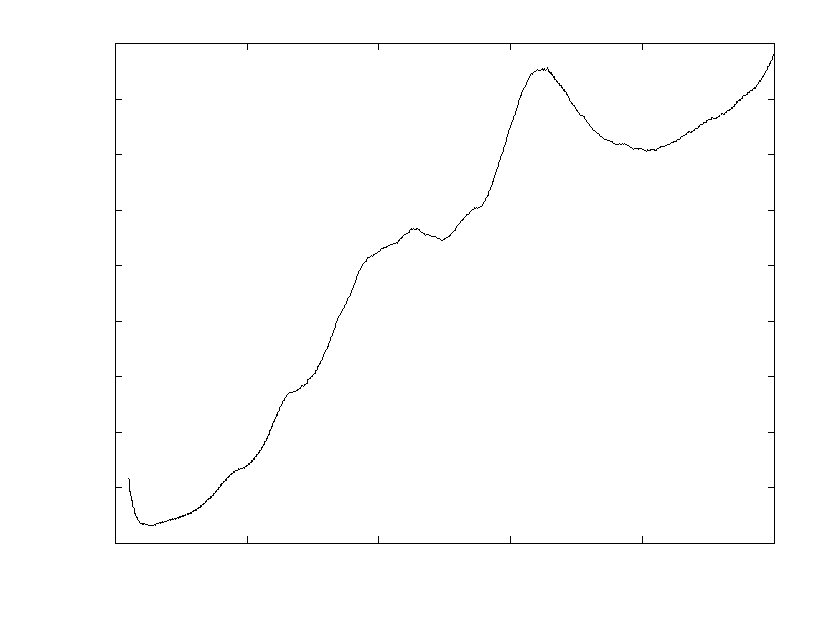
\includegraphics{Accel}}%
    \gplfronttext
  \end{picture}%
\endgroup

\label{fig:accel}
\caption{Average acceleration of particles throughout the simulation.}
\end{figure}

\begin{figure}[htbp]
\centering
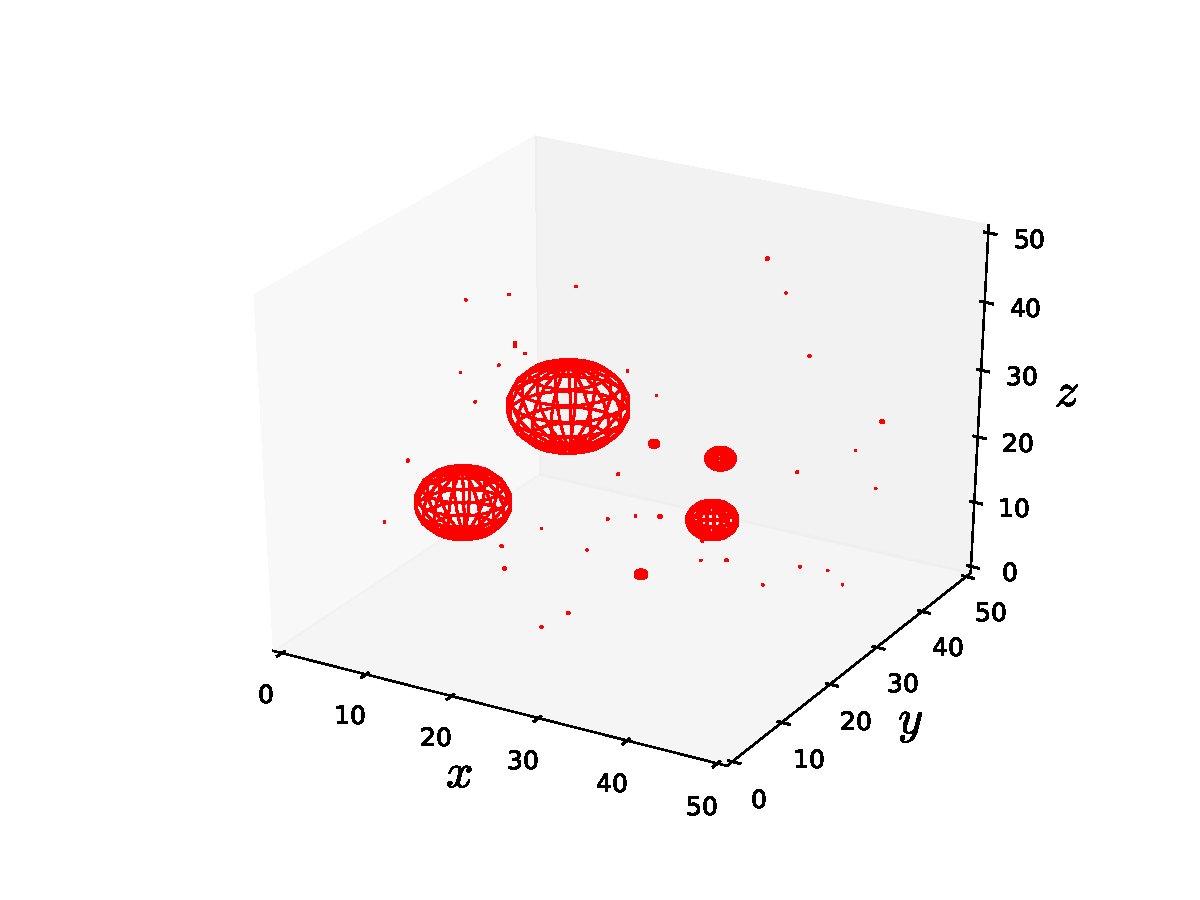
\includegraphics{Control_Groups.pdf}
\caption{Groups}
\label{fig:groups}
\end{figure}


\begin{figure}[htbp]
\centering
% GNUPLOT: LaTeX picture with Postscript
\begingroup
  \makeatletter
  \providecommand\color[2][]{%
    \GenericError{(gnuplot) \space\space\space\@spaces}{%
      Package color not loaded in conjunction with
      terminal option `colourtext'%
    }{See the gnuplot documentation for explanation.%
    }{Either use 'blacktext' in gnuplot or load the package
      color.sty in LaTeX.}%
    \renewcommand\color[2][]{}%
  }%
  \providecommand\includegraphics[2][]{%
    \GenericError{(gnuplot) \space\space\space\@spaces}{%
      Package graphicx or graphics not loaded%
    }{See the gnuplot documentation for explanation.%
    }{The gnuplot epslatex terminal needs graphicx.sty or graphics.sty.}%
    \renewcommand\includegraphics[2][]{}%
  }%
  \providecommand\rotatebox[2]{#2}%
  \@ifundefined{ifGPcolor}{%
    \newif\ifGPcolor
    \GPcolorfalse
  }{}%
  \@ifundefined{ifGPblacktext}{%
    \newif\ifGPblacktext
    \GPblacktexttrue
  }{}%
  % define a \g@addto@macro without @ in the name:
  \let\gplgaddtomacro\g@addto@macro
  % define empty templates for all commands taking text:
  \gdef\gplbacktext{}%
  \gdef\gplfronttext{}%
  \makeatother
  \ifGPblacktext
    % no textcolor at all
    \def\colorrgb#1{}%
    \def\colorgray#1{}%
  \else
    % gray or color?
    \ifGPcolor
      \def\colorrgb#1{\color[rgb]{#1}}%
      \def\colorgray#1{\color[gray]{#1}}%
      \expandafter\def\csname LTw\endcsname{\color{white}}%
      \expandafter\def\csname LTb\endcsname{\color{black}}%
      \expandafter\def\csname LTa\endcsname{\color{black}}%
      \expandafter\def\csname LT0\endcsname{\color[rgb]{1,0,0}}%
      \expandafter\def\csname LT1\endcsname{\color[rgb]{0,1,0}}%
      \expandafter\def\csname LT2\endcsname{\color[rgb]{0,0,1}}%
      \expandafter\def\csname LT3\endcsname{\color[rgb]{1,0,1}}%
      \expandafter\def\csname LT4\endcsname{\color[rgb]{0,1,1}}%
      \expandafter\def\csname LT5\endcsname{\color[rgb]{1,1,0}}%
      \expandafter\def\csname LT6\endcsname{\color[rgb]{0,0,0}}%
      \expandafter\def\csname LT7\endcsname{\color[rgb]{1,0.3,0}}%
      \expandafter\def\csname LT8\endcsname{\color[rgb]{0.5,0.5,0.5}}%
    \else
      % gray
      \def\colorrgb#1{\color{black}}%
      \def\colorgray#1{\color[gray]{#1}}%
      \expandafter\def\csname LTw\endcsname{\color{white}}%
      \expandafter\def\csname LTb\endcsname{\color{black}}%
      \expandafter\def\csname LTa\endcsname{\color{black}}%
      \expandafter\def\csname LT0\endcsname{\color{black}}%
      \expandafter\def\csname LT1\endcsname{\color{black}}%
      \expandafter\def\csname LT2\endcsname{\color{black}}%
      \expandafter\def\csname LT3\endcsname{\color{black}}%
      \expandafter\def\csname LT4\endcsname{\color{black}}%
      \expandafter\def\csname LT5\endcsname{\color{black}}%
      \expandafter\def\csname LT6\endcsname{\color{black}}%
      \expandafter\def\csname LT7\endcsname{\color{black}}%
      \expandafter\def\csname LT8\endcsname{\color{black}}%
    \fi
  \fi
    \setlength{\unitlength}{0.0500bp}%
    \ifx\gptboxheight\undefined%
      \newlength{\gptboxheight}%
      \newlength{\gptboxwidth}%
      \newsavebox{\gptboxtext}%
    \fi%
    \setlength{\fboxrule}{0.5pt}%
    \setlength{\fboxsep}{1pt}%
\begin{picture}(7674.00,5760.00)%
    \gplgaddtomacro\gplbacktext{%
      \csname LTb\endcsname%
      \put(1003,1433){\makebox(0,0){\strut{}$0$}}%
      \put(1350,1364){\makebox(0,0){\strut{}$0.1$}}%
      \put(1698,1294){\makebox(0,0){\strut{}$0.2$}}%
      \put(2045,1224){\makebox(0,0){\strut{}$0.3$}}%
      \put(2392,1155){\makebox(0,0){\strut{}$0.4$}}%
      \put(2740,1085){\makebox(0,0){\strut{}$0.5$}}%
      \put(3087,1015){\makebox(0,0){\strut{}$0.6$}}%
      \put(3434,946){\makebox(0,0){\strut{}$0.7$}}%
      \put(3782,876){\makebox(0,0){\strut{}$0.8$}}%
      \put(4128,806){\makebox(0,0){\strut{}$0.9$}}%
      \put(4476,737){\makebox(0,0){\strut{}$1$}}%
      \put(4685,794){\makebox(0,0){\strut{}$0$}}%
      \put(4885,914){\makebox(0,0){\strut{}$0.1$}}%
      \put(5086,1035){\makebox(0,0){\strut{}$0.2$}}%
      \put(5287,1156){\makebox(0,0){\strut{}$0.3$}}%
      \put(5487,1276){\makebox(0,0){\strut{}$0.4$}}%
      \put(5688,1397){\makebox(0,0){\strut{}$0.5$}}%
      \put(5888,1518){\makebox(0,0){\strut{}$0.6$}}%
      \put(6089,1638){\makebox(0,0){\strut{}$0.7$}}%
      \put(6289,1759){\makebox(0,0){\strut{}$0.8$}}%
      \put(6490,1880){\makebox(0,0){\strut{}$0.9$}}%
      \put(6690,2001){\makebox(0,0){\strut{}$1$}}%
      \put(972,1529){\makebox(0,0)[r]{\strut{}$0$}}%
      \put(972,1770){\makebox(0,0)[r]{\strut{}$0.1$}}%
      \put(972,2011){\makebox(0,0)[r]{\strut{}$0.2$}}%
      \put(972,2253){\makebox(0,0)[r]{\strut{}$0.3$}}%
      \put(972,2494){\makebox(0,0)[r]{\strut{}$0.4$}}%
      \put(972,2735){\makebox(0,0)[r]{\strut{}$0.5$}}%
      \put(972,2977){\makebox(0,0)[r]{\strut{}$0.6$}}%
      \put(972,3217){\makebox(0,0)[r]{\strut{}$0.7$}}%
      \put(972,3459){\makebox(0,0)[r]{\strut{}$0.8$}}%
      \put(972,3700){\makebox(0,0)[r]{\strut{}$0.9$}}%
      \put(972,3941){\makebox(0,0)[r]{\strut{}$1$}}%
      \put(174,2735){\makebox(0,0){\strut{}$z$}}%
    }%
    \gplgaddtomacro\gplfronttext{%
      \csname LTb\endcsname%
      \put(2333,879){\makebox(0,0){\strut{}$x$}}%
      \put(6442,1261){\makebox(0,0){\strut{}$y$}}%
      \put(174,2735){\makebox(0,0){\strut{}$z$}}%
      \put(7089,2580){\makebox(0,0)[l]{\strut{}$0$}}%
      \put(7089,2819){\makebox(0,0)[l]{\strut{}$1$}}%
      \put(7089,3058){\makebox(0,0)[l]{\strut{}$2$}}%
      \put(7089,3298){\makebox(0,0)[l]{\strut{}$3$}}%
      \put(7089,3537){\makebox(0,0)[l]{\strut{}$4$}}%
      \put(7089,3776){\makebox(0,0)[l]{\strut{}$5$}}%
      \put(7089,4016){\makebox(0,0)[l]{\strut{}$6$}}%
      \put(7089,4255){\makebox(0,0)[l]{\strut{}$7$}}%
      \put(7287,3477){\makebox(0,0){\strut{}$v$}}%
    }%
    \gplbacktext
    \put(0,0){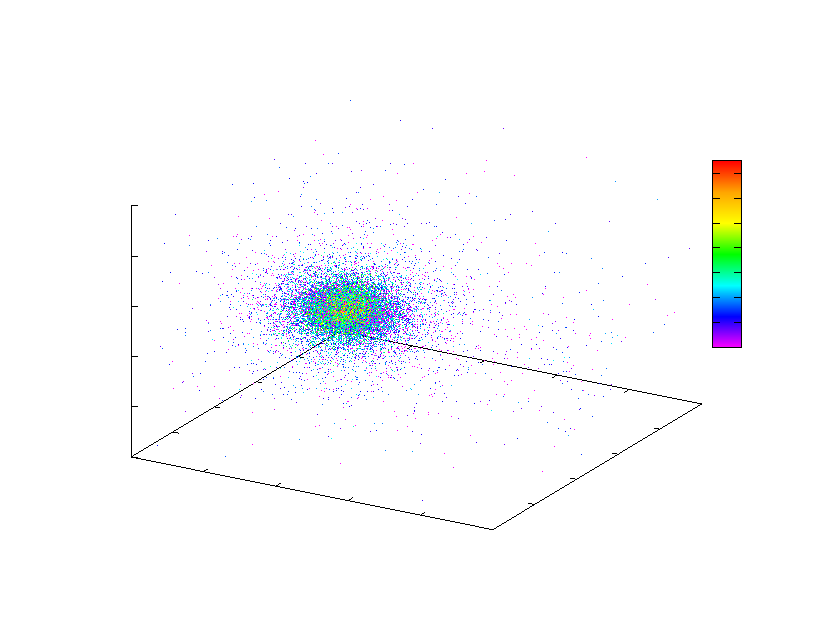
\includegraphics{1boxsize}}%
    \gplfronttext
  \end{picture}%
\endgroup

\caption{boxsize = 1}
\label{fig:1boxsize}
\end{figure}

\begin{figure}[htbp]
\centering
% GNUPLOT: LaTeX picture with Postscript
\begingroup
  \makeatletter
  \providecommand\color[2][]{%
    \GenericError{(gnuplot) \space\space\space\@spaces}{%
      Package color not loaded in conjunction with
      terminal option `colourtext'%
    }{See the gnuplot documentation for explanation.%
    }{Either use 'blacktext' in gnuplot or load the package
      color.sty in LaTeX.}%
    \renewcommand\color[2][]{}%
  }%
  \providecommand\includegraphics[2][]{%
    \GenericError{(gnuplot) \space\space\space\@spaces}{%
      Package graphicx or graphics not loaded%
    }{See the gnuplot documentation for explanation.%
    }{The gnuplot epslatex terminal needs graphicx.sty or graphics.sty.}%
    \renewcommand\includegraphics[2][]{}%
  }%
  \providecommand\rotatebox[2]{#2}%
  \@ifundefined{ifGPcolor}{%
    \newif\ifGPcolor
    \GPcolorfalse
  }{}%
  \@ifundefined{ifGPblacktext}{%
    \newif\ifGPblacktext
    \GPblacktexttrue
  }{}%
  % define a \g@addto@macro without @ in the name:
  \let\gplgaddtomacro\g@addto@macro
  % define empty templates for all commands taking text:
  \gdef\gplbacktext{}%
  \gdef\gplfronttext{}%
  \makeatother
  \ifGPblacktext
    % no textcolor at all
    \def\colorrgb#1{}%
    \def\colorgray#1{}%
  \else
    % gray or color?
    \ifGPcolor
      \def\colorrgb#1{\color[rgb]{#1}}%
      \def\colorgray#1{\color[gray]{#1}}%
      \expandafter\def\csname LTw\endcsname{\color{white}}%
      \expandafter\def\csname LTb\endcsname{\color{black}}%
      \expandafter\def\csname LTa\endcsname{\color{black}}%
      \expandafter\def\csname LT0\endcsname{\color[rgb]{1,0,0}}%
      \expandafter\def\csname LT1\endcsname{\color[rgb]{0,1,0}}%
      \expandafter\def\csname LT2\endcsname{\color[rgb]{0,0,1}}%
      \expandafter\def\csname LT3\endcsname{\color[rgb]{1,0,1}}%
      \expandafter\def\csname LT4\endcsname{\color[rgb]{0,1,1}}%
      \expandafter\def\csname LT5\endcsname{\color[rgb]{1,1,0}}%
      \expandafter\def\csname LT6\endcsname{\color[rgb]{0,0,0}}%
      \expandafter\def\csname LT7\endcsname{\color[rgb]{1,0.3,0}}%
      \expandafter\def\csname LT8\endcsname{\color[rgb]{0.5,0.5,0.5}}%
    \else
      % gray
      \def\colorrgb#1{\color{black}}%
      \def\colorgray#1{\color[gray]{#1}}%
      \expandafter\def\csname LTw\endcsname{\color{white}}%
      \expandafter\def\csname LTb\endcsname{\color{black}}%
      \expandafter\def\csname LTa\endcsname{\color{black}}%
      \expandafter\def\csname LT0\endcsname{\color{black}}%
      \expandafter\def\csname LT1\endcsname{\color{black}}%
      \expandafter\def\csname LT2\endcsname{\color{black}}%
      \expandafter\def\csname LT3\endcsname{\color{black}}%
      \expandafter\def\csname LT4\endcsname{\color{black}}%
      \expandafter\def\csname LT5\endcsname{\color{black}}%
      \expandafter\def\csname LT6\endcsname{\color{black}}%
      \expandafter\def\csname LT7\endcsname{\color{black}}%
      \expandafter\def\csname LT8\endcsname{\color{black}}%
    \fi
  \fi
    \setlength{\unitlength}{0.0500bp}%
    \ifx\gptboxheight\undefined%
      \newlength{\gptboxheight}%
      \newlength{\gptboxwidth}%
      \newsavebox{\gptboxtext}%
    \fi%
    \setlength{\fboxrule}{0.5pt}%
    \setlength{\fboxsep}{1pt}%
\begin{picture}(7674.00,5760.00)%
    \gplgaddtomacro\gplbacktext{%
      \csname LTb\endcsname%
      \put(1003,1433){\makebox(0,0){\strut{}$0$}}%
      \put(1698,1294){\makebox(0,0){\strut{}$10$}}%
      \put(2392,1155){\makebox(0,0){\strut{}$20$}}%
      \put(3087,1015){\makebox(0,0){\strut{}$30$}}%
      \put(3782,876){\makebox(0,0){\strut{}$40$}}%
      \put(4476,737){\makebox(0,0){\strut{}$50$}}%
      \put(4685,794){\makebox(0,0){\strut{}$0$}}%
      \put(5086,1035){\makebox(0,0){\strut{}$10$}}%
      \put(5487,1276){\makebox(0,0){\strut{}$20$}}%
      \put(5888,1518){\makebox(0,0){\strut{}$30$}}%
      \put(6289,1759){\makebox(0,0){\strut{}$40$}}%
      \put(6690,2001){\makebox(0,0){\strut{}$50$}}%
      \put(972,1529){\makebox(0,0)[r]{\strut{}$0$}}%
      \put(972,2011){\makebox(0,0)[r]{\strut{}$10$}}%
      \put(972,2494){\makebox(0,0)[r]{\strut{}$20$}}%
      \put(972,2977){\makebox(0,0)[r]{\strut{}$30$}}%
      \put(972,3459){\makebox(0,0)[r]{\strut{}$40$}}%
      \put(972,3941){\makebox(0,0)[r]{\strut{}$50$}}%
      \put(174,2735){\makebox(0,0){\strut{}$z$}}%
    }%
    \gplgaddtomacro\gplfronttext{%
      \csname LTb\endcsname%
      \put(2333,879){\makebox(0,0){\strut{}$x$}}%
      \put(6442,1261){\makebox(0,0){\strut{}$y$}}%
      \put(174,2735){\makebox(0,0){\strut{}$z$}}%
      \put(7089,2580){\makebox(0,0)[l]{\strut{}$0$}}%
      \put(7089,2939){\makebox(0,0)[l]{\strut{}$20$}}%
      \put(7089,3298){\makebox(0,0)[l]{\strut{}$40$}}%
      \put(7089,3657){\makebox(0,0)[l]{\strut{}$60$}}%
      \put(7089,4016){\makebox(0,0)[l]{\strut{}$80$}}%
      \put(7089,4375){\makebox(0,0)[l]{\strut{}$100$}}%
      \put(7551,3477){\makebox(0,0){\strut{}$v$}}%
    }%
    \gplbacktext
    \put(0,0){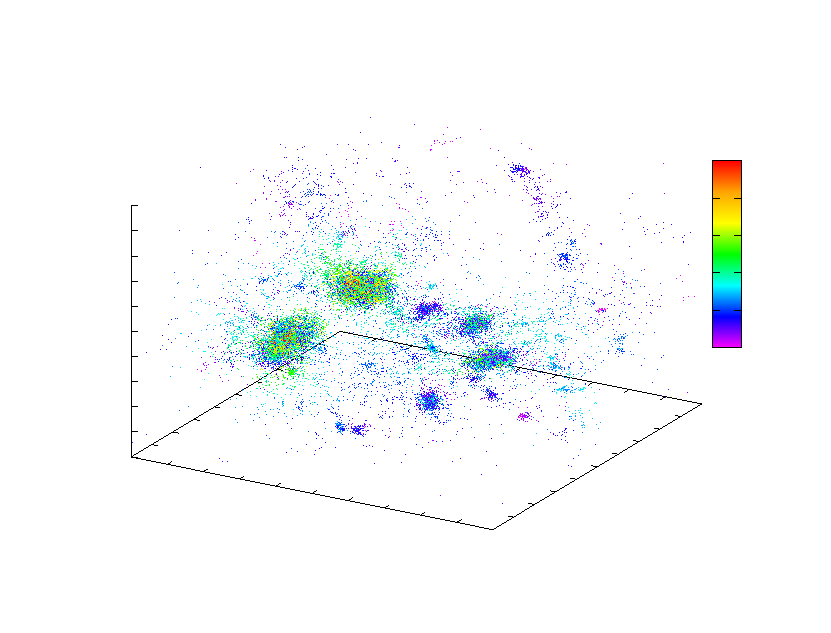
\includegraphics{3mass}}%
    \gplfronttext
  \end{picture}%
\endgroup

\caption{$\Omega_m = 3.0$, $\Omega_k = \Omega_\Lambda = 0$}
\label{fig:3mass}
\end{figure}

\begin{figure}[htbp]
\centering
% GNUPLOT: LaTeX picture with Postscript
\begingroup
  \makeatletter
  \providecommand\color[2][]{%
    \GenericError{(gnuplot) \space\space\space\@spaces}{%
      Package color not loaded in conjunction with
      terminal option `colourtext'%
    }{See the gnuplot documentation for explanation.%
    }{Either use 'blacktext' in gnuplot or load the package
      color.sty in LaTeX.}%
    \renewcommand\color[2][]{}%
  }%
  \providecommand\includegraphics[2][]{%
    \GenericError{(gnuplot) \space\space\space\@spaces}{%
      Package graphicx or graphics not loaded%
    }{See the gnuplot documentation for explanation.%
    }{The gnuplot epslatex terminal needs graphicx.sty or graphics.sty.}%
    \renewcommand\includegraphics[2][]{}%
  }%
  \providecommand\rotatebox[2]{#2}%
  \@ifundefined{ifGPcolor}{%
    \newif\ifGPcolor
    \GPcolorfalse
  }{}%
  \@ifundefined{ifGPblacktext}{%
    \newif\ifGPblacktext
    \GPblacktexttrue
  }{}%
  % define a \g@addto@macro without @ in the name:
  \let\gplgaddtomacro\g@addto@macro
  % define empty templates for all commands taking text:
  \gdef\gplbacktext{}%
  \gdef\gplfronttext{}%
  \makeatother
  \ifGPblacktext
    % no textcolor at all
    \def\colorrgb#1{}%
    \def\colorgray#1{}%
  \else
    % gray or color?
    \ifGPcolor
      \def\colorrgb#1{\color[rgb]{#1}}%
      \def\colorgray#1{\color[gray]{#1}}%
      \expandafter\def\csname LTw\endcsname{\color{white}}%
      \expandafter\def\csname LTb\endcsname{\color{black}}%
      \expandafter\def\csname LTa\endcsname{\color{black}}%
      \expandafter\def\csname LT0\endcsname{\color[rgb]{1,0,0}}%
      \expandafter\def\csname LT1\endcsname{\color[rgb]{0,1,0}}%
      \expandafter\def\csname LT2\endcsname{\color[rgb]{0,0,1}}%
      \expandafter\def\csname LT3\endcsname{\color[rgb]{1,0,1}}%
      \expandafter\def\csname LT4\endcsname{\color[rgb]{0,1,1}}%
      \expandafter\def\csname LT5\endcsname{\color[rgb]{1,1,0}}%
      \expandafter\def\csname LT6\endcsname{\color[rgb]{0,0,0}}%
      \expandafter\def\csname LT7\endcsname{\color[rgb]{1,0.3,0}}%
      \expandafter\def\csname LT8\endcsname{\color[rgb]{0.5,0.5,0.5}}%
    \else
      % gray
      \def\colorrgb#1{\color{black}}%
      \def\colorgray#1{\color[gray]{#1}}%
      \expandafter\def\csname LTw\endcsname{\color{white}}%
      \expandafter\def\csname LTb\endcsname{\color{black}}%
      \expandafter\def\csname LTa\endcsname{\color{black}}%
      \expandafter\def\csname LT0\endcsname{\color{black}}%
      \expandafter\def\csname LT1\endcsname{\color{black}}%
      \expandafter\def\csname LT2\endcsname{\color{black}}%
      \expandafter\def\csname LT3\endcsname{\color{black}}%
      \expandafter\def\csname LT4\endcsname{\color{black}}%
      \expandafter\def\csname LT5\endcsname{\color{black}}%
      \expandafter\def\csname LT6\endcsname{\color{black}}%
      \expandafter\def\csname LT7\endcsname{\color{black}}%
      \expandafter\def\csname LT8\endcsname{\color{black}}%
    \fi
  \fi
    \setlength{\unitlength}{0.0500bp}%
    \ifx\gptboxheight\undefined%
      \newlength{\gptboxheight}%
      \newlength{\gptboxwidth}%
      \newsavebox{\gptboxtext}%
    \fi%
    \setlength{\fboxrule}{0.5pt}%
    \setlength{\fboxsep}{1pt}%
\begin{picture}(7674.00,5760.00)%
    \gplgaddtomacro\gplbacktext{%
      \csname LTb\endcsname%
      \put(1003,1433){\makebox(0,0){\strut{}$0$}}%
      \put(1698,1294){\makebox(0,0){\strut{}$10$}}%
      \put(2392,1155){\makebox(0,0){\strut{}$20$}}%
      \put(3087,1015){\makebox(0,0){\strut{}$30$}}%
      \put(3782,876){\makebox(0,0){\strut{}$40$}}%
      \put(4476,737){\makebox(0,0){\strut{}$50$}}%
      \put(4685,794){\makebox(0,0){\strut{}$0$}}%
      \put(5086,1035){\makebox(0,0){\strut{}$10$}}%
      \put(5487,1276){\makebox(0,0){\strut{}$20$}}%
      \put(5888,1518){\makebox(0,0){\strut{}$30$}}%
      \put(6289,1759){\makebox(0,0){\strut{}$40$}}%
      \put(6690,2001){\makebox(0,0){\strut{}$50$}}%
      \put(972,1529){\makebox(0,0)[r]{\strut{}$0$}}%
      \put(972,2011){\makebox(0,0)[r]{\strut{}$10$}}%
      \put(972,2494){\makebox(0,0)[r]{\strut{}$20$}}%
      \put(972,2977){\makebox(0,0)[r]{\strut{}$30$}}%
      \put(972,3459){\makebox(0,0)[r]{\strut{}$40$}}%
      \put(972,3941){\makebox(0,0)[r]{\strut{}$50$}}%
      \put(174,2735){\makebox(0,0){\strut{}$z$}}%
    }%
    \gplgaddtomacro\gplfronttext{%
      \csname LTb\endcsname%
      \put(2333,879){\makebox(0,0){\strut{}$x$}}%
      \put(6442,1261){\makebox(0,0){\strut{}$y$}}%
      \put(174,2735){\makebox(0,0){\strut{}$z$}}%
      \put(7089,2580){\makebox(0,0)[l]{\strut{}$0$}}%
      \put(7089,2939){\makebox(0,0)[l]{\strut{}$2$}}%
      \put(7089,3298){\makebox(0,0)[l]{\strut{}$4$}}%
      \put(7089,3657){\makebox(0,0)[l]{\strut{}$6$}}%
      \put(7089,4016){\makebox(0,0)[l]{\strut{}$8$}}%
      \put(7089,4375){\makebox(0,0)[l]{\strut{}$10$}}%
      \put(7419,3477){\makebox(0,0){\strut{}$v$}}%
    }%
    \gplbacktext
    \put(0,0){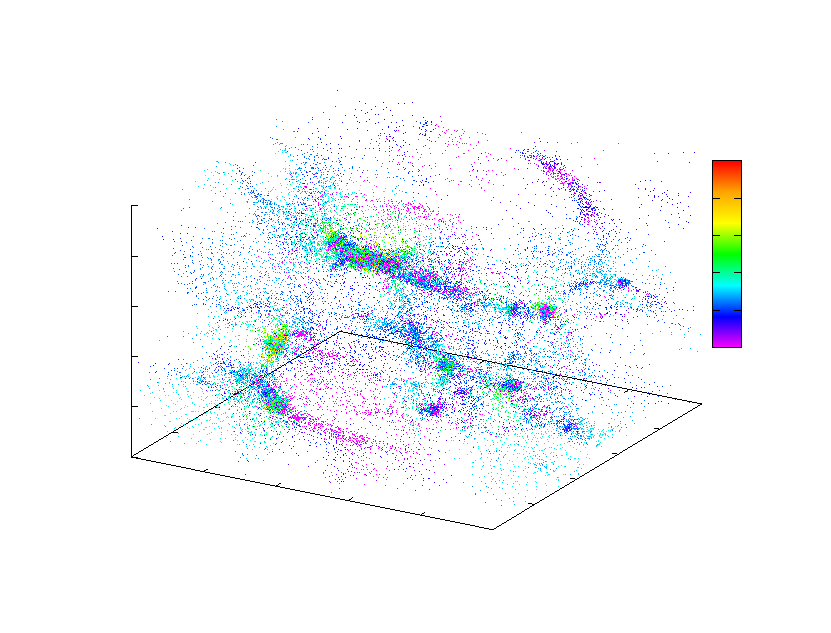
\includegraphics{1Ncells}}%
    \gplfronttext
  \end{picture}%
\endgroup

\caption{$N_c = n^{1/3}$}
\label{fig:1ncells}
\end{figure}

\begin{figure}[htbp]
\centering
% GNUPLOT: LaTeX picture with Postscript
\begingroup
  \makeatletter
  \providecommand\color[2][]{%
    \GenericError{(gnuplot) \space\space\space\@spaces}{%
      Package color not loaded in conjunction with
      terminal option `colourtext'%
    }{See the gnuplot documentation for explanation.%
    }{Either use 'blacktext' in gnuplot or load the package
      color.sty in LaTeX.}%
    \renewcommand\color[2][]{}%
  }%
  \providecommand\includegraphics[2][]{%
    \GenericError{(gnuplot) \space\space\space\@spaces}{%
      Package graphicx or graphics not loaded%
    }{See the gnuplot documentation for explanation.%
    }{The gnuplot epslatex terminal needs graphicx.sty or graphics.sty.}%
    \renewcommand\includegraphics[2][]{}%
  }%
  \providecommand\rotatebox[2]{#2}%
  \@ifundefined{ifGPcolor}{%
    \newif\ifGPcolor
    \GPcolorfalse
  }{}%
  \@ifundefined{ifGPblacktext}{%
    \newif\ifGPblacktext
    \GPblacktexttrue
  }{}%
  % define a \g@addto@macro without @ in the name:
  \let\gplgaddtomacro\g@addto@macro
  % define empty templates for all commands taking text:
  \gdef\gplbacktext{}%
  \gdef\gplfronttext{}%
  \makeatother
  \ifGPblacktext
    % no textcolor at all
    \def\colorrgb#1{}%
    \def\colorgray#1{}%
  \else
    % gray or color?
    \ifGPcolor
      \def\colorrgb#1{\color[rgb]{#1}}%
      \def\colorgray#1{\color[gray]{#1}}%
      \expandafter\def\csname LTw\endcsname{\color{white}}%
      \expandafter\def\csname LTb\endcsname{\color{black}}%
      \expandafter\def\csname LTa\endcsname{\color{black}}%
      \expandafter\def\csname LT0\endcsname{\color[rgb]{1,0,0}}%
      \expandafter\def\csname LT1\endcsname{\color[rgb]{0,1,0}}%
      \expandafter\def\csname LT2\endcsname{\color[rgb]{0,0,1}}%
      \expandafter\def\csname LT3\endcsname{\color[rgb]{1,0,1}}%
      \expandafter\def\csname LT4\endcsname{\color[rgb]{0,1,1}}%
      \expandafter\def\csname LT5\endcsname{\color[rgb]{1,1,0}}%
      \expandafter\def\csname LT6\endcsname{\color[rgb]{0,0,0}}%
      \expandafter\def\csname LT7\endcsname{\color[rgb]{1,0.3,0}}%
      \expandafter\def\csname LT8\endcsname{\color[rgb]{0.5,0.5,0.5}}%
    \else
      % gray
      \def\colorrgb#1{\color{black}}%
      \def\colorgray#1{\color[gray]{#1}}%
      \expandafter\def\csname LTw\endcsname{\color{white}}%
      \expandafter\def\csname LTb\endcsname{\color{black}}%
      \expandafter\def\csname LTa\endcsname{\color{black}}%
      \expandafter\def\csname LT0\endcsname{\color{black}}%
      \expandafter\def\csname LT1\endcsname{\color{black}}%
      \expandafter\def\csname LT2\endcsname{\color{black}}%
      \expandafter\def\csname LT3\endcsname{\color{black}}%
      \expandafter\def\csname LT4\endcsname{\color{black}}%
      \expandafter\def\csname LT5\endcsname{\color{black}}%
      \expandafter\def\csname LT6\endcsname{\color{black}}%
      \expandafter\def\csname LT7\endcsname{\color{black}}%
      \expandafter\def\csname LT8\endcsname{\color{black}}%
    \fi
  \fi
    \setlength{\unitlength}{0.0500bp}%
    \ifx\gptboxheight\undefined%
      \newlength{\gptboxheight}%
      \newlength{\gptboxwidth}%
      \newsavebox{\gptboxtext}%
    \fi%
    \setlength{\fboxrule}{0.5pt}%
    \setlength{\fboxsep}{1pt}%
\begin{picture}(7674.00,5760.00)%
    \gplgaddtomacro\gplbacktext{%
      \csname LTb\endcsname%
      \put(1003,1433){\makebox(0,0){\strut{}$0$}}%
      \put(1698,1294){\makebox(0,0){\strut{}$10$}}%
      \put(2392,1155){\makebox(0,0){\strut{}$20$}}%
      \put(3087,1015){\makebox(0,0){\strut{}$30$}}%
      \put(3782,876){\makebox(0,0){\strut{}$40$}}%
      \put(4476,737){\makebox(0,0){\strut{}$50$}}%
      \put(4685,794){\makebox(0,0){\strut{}$0$}}%
      \put(5086,1035){\makebox(0,0){\strut{}$10$}}%
      \put(5487,1276){\makebox(0,0){\strut{}$20$}}%
      \put(5888,1518){\makebox(0,0){\strut{}$30$}}%
      \put(6289,1759){\makebox(0,0){\strut{}$40$}}%
      \put(6690,2001){\makebox(0,0){\strut{}$50$}}%
      \put(972,1529){\makebox(0,0)[r]{\strut{}$0$}}%
      \put(972,2011){\makebox(0,0)[r]{\strut{}$10$}}%
      \put(972,2494){\makebox(0,0)[r]{\strut{}$20$}}%
      \put(972,2977){\makebox(0,0)[r]{\strut{}$30$}}%
      \put(972,3459){\makebox(0,0)[r]{\strut{}$40$}}%
      \put(972,3941){\makebox(0,0)[r]{\strut{}$50$}}%
      \put(174,2735){\makebox(0,0){\strut{}$z$}}%
    }%
    \gplgaddtomacro\gplfronttext{%
      \csname LTb\endcsname%
      \put(2333,879){\makebox(0,0){\strut{}$x$}}%
      \put(6442,1261){\makebox(0,0){\strut{}$y$}}%
      \put(174,2735){\makebox(0,0){\strut{}$z$}}%
      \put(7089,2580){\makebox(0,0)[l]{\strut{}$0$}}%
      \put(7089,2939){\makebox(0,0)[l]{\strut{}$10$}}%
      \put(7089,3298){\makebox(0,0)[l]{\strut{}$20$}}%
      \put(7089,3657){\makebox(0,0)[l]{\strut{}$30$}}%
      \put(7089,4016){\makebox(0,0)[l]{\strut{}$40$}}%
      \put(7089,4375){\makebox(0,0)[l]{\strut{}$50$}}%
      \put(7419,3477){\makebox(0,0){\strut{}$v$}}%
    }%
    \gplbacktext
    \put(0,0){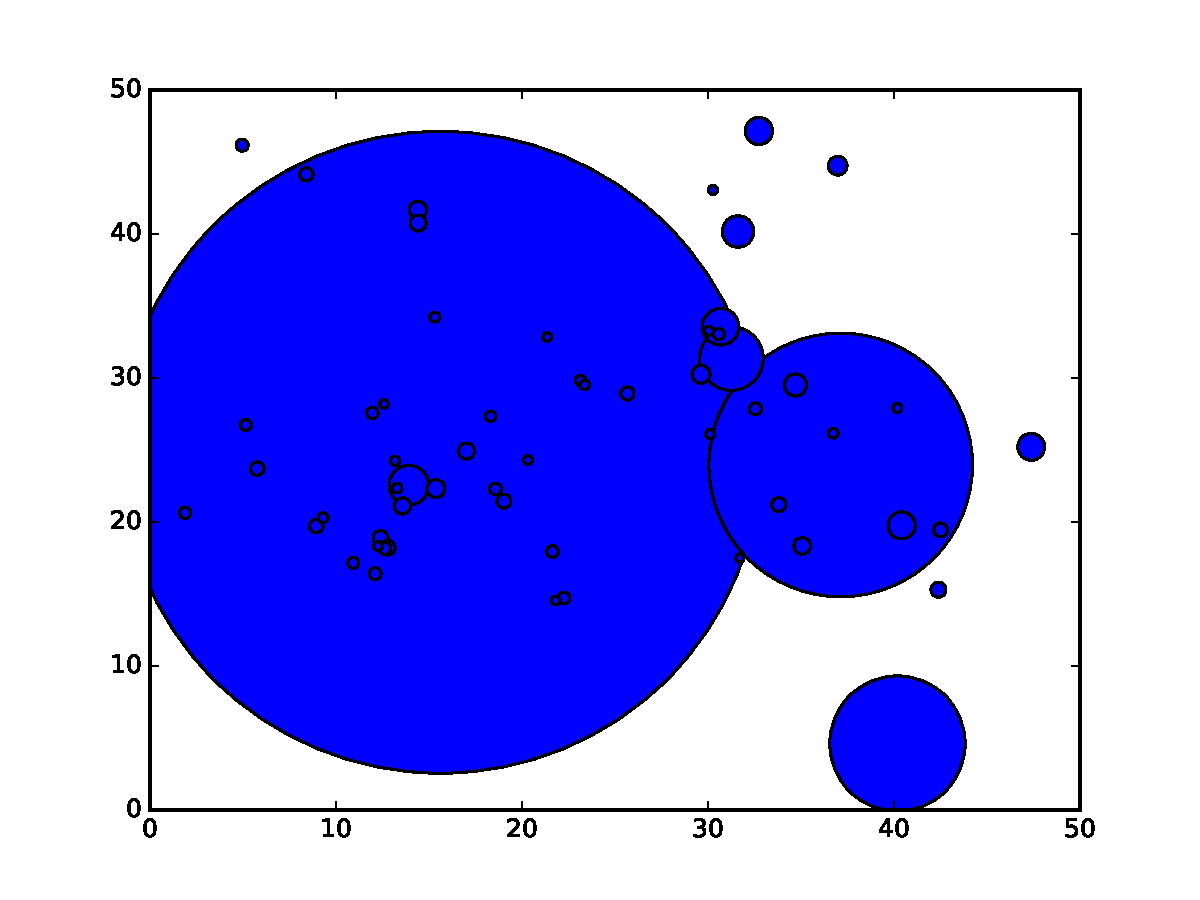
\includegraphics{N64}}%
    \gplfronttext
  \end{picture}%
\endgroup

\caption{$n = 64^3$}
\label{fig:n64}
\end{figure}




\end{document}
